\chapter{Applying analytics to development practices}~\label{chapter-applying-analytics-to-development-practices}
Analytics data is based on the software being used, so the software needs to be created and able to run before relevant data is generated.

Analytics, such as user-journeys, can help to answer questions about the usage of the software. They help establish \emph{what-is}. As we understand more about what-is we can then consider \emph{what-would-be-better} and do gap analysis between what-is and what-would-be-better.

Various data can be potentially collected. What can be collected depends on the observation mechanisms. The choices of observation mechanisms within an app are made by developers or their stakeholders. Observation may be within an app or external to it, for instance by the operating system as Google Android does~\footnote{There are other custom versions of Android, for instance used in Amazon Kindle Fire devices.}. Within an app the observation may focus at a single layer, for instance the visual user interface, or several.

\section{3 layers of an app}
\begin{figure}[ht]
    \begin{minipage}{\textwidth}
    \centering
    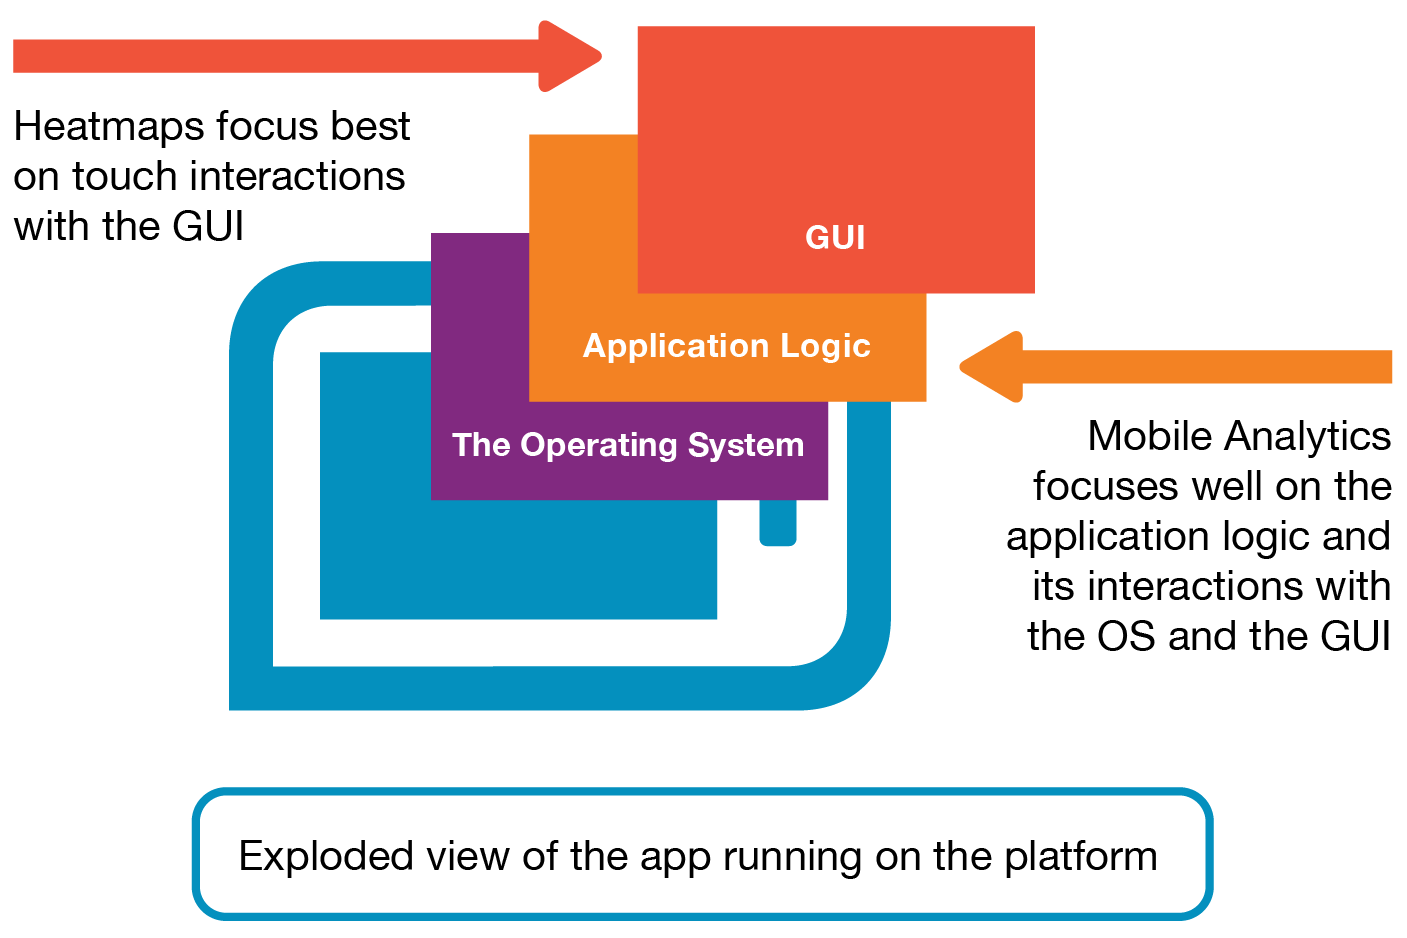
\includegraphics[width=10cm]{images/mobile-analytics-playbook/3-layers.png}
    \caption[Three layers of an app]{Three layers of an app~\footnote{Image credit: First published in the Mobile Analytics Playbook~\cite{harty_aymer_playbook_2016}}.}
    \label{fig:3-layers}
    \end{minipage}
\end{figure}

Figure \ref{fig:3-layers} illustrates three primary observation points, or layers, for a mobile app. 

The Graphical User Interface (GUI) % SHOULD-DO add to glossary.
can be visually observed by sighted users, it can also be observed by Accessibility software, and test automation tools, \emph{etc.} externally to the app. It can also be observed from within the app, for instance through using software known as \emph{heatmapping} that records the screens and the touch interactions performed by users of that screen. One of the the more popular, mature heatmapping offerings is from AppSee~\footnote{\url{  https://www.appbrain.com/stats/libraries/details/appsee/appsee}}, nonetheless they are only used in a small minority of mobile apps.

\begin{figure}[ht]
    \centering
    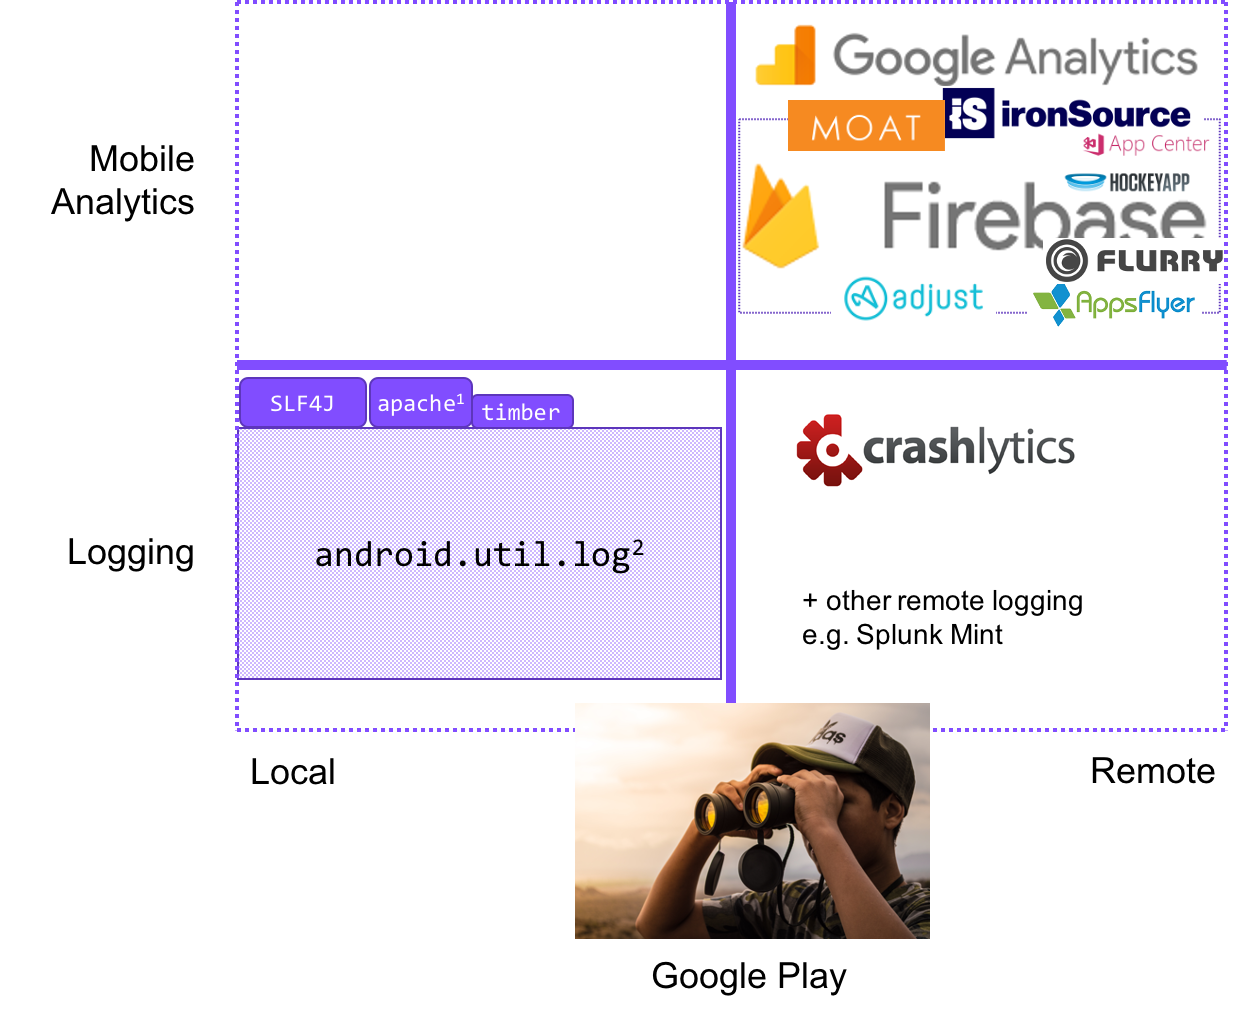
\includegraphics[width=12cm]{images/matrix-of-logging.png}
    \caption{Matrix of logging}
    \label{fig:matrix-of-logging}
\end{figure}

The application may incorporate logging and/or mobile analytics. Logging in mobile apps is often used locally, by developers independently of other mechanisms. Figure \ref{fig:matrix-of-logging} illustrates a matrix of logging, where logging and mobile analytics are on the Y axis and local and remote on the X axis. Google Play is an external observer of data recorded in device logs. Data collection runs locally and is sent to Google servers where Google analyses the data and provides reports to developers for their apps.

As an observation the vast majority of Android developers use the default inbuilt logging library \texttt{android.util.log} and choose one or more of Google's analytics offerings (which include Firebase and Crashlytics). A commercial organisation provides current statistics for third-party logging libraries~\footnote{Logging libraries (note the default library is not tracked at the time of writing~\url{https://www.appbrain.com/stats/libraries/tag/logging/logging-libraries}}, crash libraries~\footnote{\url{https://www.appbrain.com/stats/libraries/tag/crash-reporting/android-crash-reporting-libraries}} and mobile analytics~\footnote{\url{https://www.appbrain.com/stats/libraries/tag/analytics/android-analytics-libraries}}. Some apps have several of these libraries so counts may exceed 100\% in their reports.

\begin{itemize}
    \item Logging: enables developers to understand what their software is doing. The practice is commonplace across many software domains including mobile apps, and each platform and language includes a standard method of generating log messages. These messages tend to be small and intended for immediate, local consumption. On Android when developers use the standard logging library (\texttt{android.util.log}) their log messages are written to a shared circular log file on a device. Some privileged Android software is able to read these shared logs, developers can also read them using standard Android development tools \emph{e.g.} \texttt{adb logcat} providing they are connected to the device with the log file. Older versions of Android allowed apps to read the full contents, more recently apps are restricted to only the log messages they wrote unless they are granted the relevant permission by Google and the user. 
    In other domains \emph{e.g.} web servers, infrastructure software, and many others, logging is used for production monitoring, fault-finding and analysis. A minority of mobile app developers use remote logging.
    \item Mobile analytics, can extend and scale logging. For mobile analytics, a minority of developers incorporate custom implementations, however the vast majority who use analytics do so through using third-party analytics libraries such as Google Firebase Analytics, details of the current usage of analytics libraries are provided by AppBrain~\footnote{\url{https://www.appbrain.com/stats/libraries/tag/analytics/android-analytics-libraries}}.
\end{itemize}

Similar to the concept of black box testing (where software's behaviour is observed and assessed without knowing the internals), external software can observe the behaviours of apps. Google have developed and integrated software that monitors apps running in Google approved versions of Android. The data is collected per device and provided automatically to Google servers if the device has the relevant settings enabled~\cite{google_play_share_usage_and_diagnostics_info_with_google}. This data is processed by Google who provide some portions of the data to the registered developers of that app in the Google Play Store.

\emph{Idea for expansion:} Drop-off in data for a population  c.f. marketing funnels, funnels for shopping carts, etc.

\section{Overview of applying analytics to development practices}
\begin{itemize}
    \item Decide whether to use any existing, pre-provided analytics. This includes \emph{passive analytics} (gathered without the developers needing to actively include analytics tools in their app). It may also include analytics provided as a side-effect of incorporating libraries into the app without the developers needing to add code to record additional information. 
    \item Decide whether to incorporate analytics into the app, and if so what data to collect, which analytics library/libraries to incorporate and the many associated aspects we will cover in this chapter.
    \item Consider whether and how to test analytics and whether to filter [out] analytics during automated and internal testing.
    \item Use and analyse the analytics data from the app and the platform (where available).
    \item Triage and prioritise potential issues reported from external sources (pre-launch testing, new releases, active mainstream releases, etc.)
\end{itemize}

\subsection{Levels of engagement}
Continuum of levels of engagement, or commitment, by developers:
\begin{enumerate}
    \setcounter{enumi}{-1} % unexpectedly this sets the first item in this list to zero.
    \item No analytics incorporated in the development process. If they exist, they're ignored.
    \item Passive analytics incorporated, app does not contain any crash recording, remote logging, or other mobile analytics libraries.
    \item App incorporates one or more of the above mentioned libraries, initialises them where necessary but does not add any other additional calls to the libraries.
    \item App incorporates additional code to call one or methods using the APIs (\emph{etc.} if other mechanisms are available).
\end{enumerate}

In terms of incorporating analytics, 
\subsection{Incorporating passive analytics e.g. Google Play Console to development practices}
\href{google_play_console_section}{\emph{\nameref{google_play_console_section}}} provides developers with a variety of reports on the performance of their Android app. Developers can integrate and incorporate the passive analytics Google provides through the various reports in order to a) better understand how their app is doing b) change their app so it performs better as reported by these reports.

Here are the reports in the most likely order of being generated if developers follow various recommendations made by Google, \emph{i.e.} to create and take advantage of test releases and use release management tools when rolling out a release of their Android app into production.

\begin{enumerate}
    \item \textbf{Pre-launch reports}: 
    \item \textbf{Alpha and Beta channels}:
    \item \textbf{Release Management}: Note this fits with existing research in release management by Shane Mcintosh and Guenther Ruhe, and others.
    
    \item (the app) \textbf{Dashboard, including User Feedback}:
    \item \textbf{Android Vitals}:
\end{enumerate}

\subsubsection{Privacy and Responsibilities for using passive analytics}
For passive analytics the developer does not actively choose what to collect or how it's collected, therefore they are constrained by whoever, or whatever if we discount the people involved in deciding what to collect, etc. and assume algorithms such as AI determine the data. Google, at least, is careful to only share non PII % MUST_DO expand and add PII to the Glossary.
data and with a few exceptions limits reports to populations that exceed thresholds determined by Google internally. %MUST_DO add reference to Google Help article(s).

Nonetheless, I recommend developers consider ethical and legal responsibilities if they discover that sensitive and other PII data is being collected through the passive analytics. This may include avoiding reports with such data in them and also reporting the concerns to upstream providers of analytics (and where appropriate internal and external legal authorities).

\section{An aside on packaging mobile apps}
Mobile apps are a bit like snails, who carry everything with them in their shell, well actually in their application binary package (known as an APK~\footnote{Android Package Kit\url{https://en.wikipedia.org/wiki/Android_application_package}} file). This includes whichever libraries they use. Therefore, when developers want to include pre-packaged support for crash-reporting and/or mobile analytics, the development team need to incorporate the relevant software libraries in their application binary package. These libraries are therefore distributed as an intrinsic part of an app and installed seamlessly with the main application onto a user's device.

\section{Applying a crash-reporting library}
As mentioned in the section on packaging mobile apps, crash-reporting libraries need to be incorporated into an application before they can be used. Generally~\footnote{A small minority of developers may follow other practices, nonetheless the principles mentioned here still apply}, the developer adds a few configuration lines to their application's build file (in \texttt{app/build.gradle} for Android apps) and also several lines of code to initialise the library when the application starts. These install the library as the global crash handler for the app, each time the app is started the library is initialised. 

When the library is initialised, it may perform various actions such recording details of the operating system release, the model of device, \emph{etc.}. They may also perform house-keeping activities, for instance Crashlytics transmits crash reports from previous sessions.

Some crash-reporting libraries offer developers an API to add \emph{breadcrumbs} at run-time. If/when a crash occurs and is reported, the immediately preceding breadcrumb data may help developers piece together possible causes for a particular crash.

Some crash-reporting libraries offer developers a mechanism to report non-fatal crashes: caught exceptions. These would be handled by the application yet be considered noteworthy and worthy of analysis by the development team. A good example of a library that includes support for non-fatal crash reporting is the popular Crashlytics offering.  

\subsection{Testing crash-reporting}
\begin{itemize}
    \item Sanity test
    \item Latency
\end{itemize}

Testing a system intended to measure quality may adversely affect their rating of your apps and potentially even their willingness to accept you in their system. \emph{c.f.} credit checks may adversely affect your credit score score~\footnote{\url{https://www.experian.co.uk/consumer/guides/searches-and-credit-checks.html}}. The system may not distinguish between your testing of the measurement system and those experienced by end users of the software. Google is adamant they will not accept Android apps that crash: ~\emph{``\textbf{Broken Functionality} We don’t allow apps that crash, force close, freeze, or otherwise function abnormally."}~\cite{google_play_developer_policy_center}.

\section{Designing the messages}
This section applies to messages that an app could emit regardless of the conduit (\emph{i.e.} it applies to logging and using mobile analytics).

\emph{Related concepts}: The uneven U, computer protocols (layers, formatting, and contents), structured messages, what to log. %MUST_DO expand this section.

Developers have control over what to log, how, and when to generate the log messages. They may be constrained in various ways by APIs, message lengths, encoding, and formats, access to messages, and when messages will be transmitted, \emph{etc.} 

It is possible to test the constraints, for instance by writing custom automated tests and/or apps that generate a variety of messages where the outputs are checked somehow. The checking may be partly or completely performed programmatically (we did some unpublished research in this area in 2018).

The purpose of the message may differ in the type and level of information it is intended to convey. Some messages may contain low-level, or detailed, error messages intended to help improve the technical aspects of the software to make the software more robust. Other messages may aim to communicate intent, completion of a task, activity or user-journey in the software. For example, IBM published a paper about software called CX Mobile that aims to record and visualise user journeys for iOS and Android apps~\cite{hu_tealeaf_cxmobile}.

\section{Designing logging}
\subsection{Testing logging}

\section{Designing in-app analytics}
\subsection{Testing in-app analytics}

\section{An aside on 'pre-launch reports'}
Google provide a free service called pre-launch reports~\cite{google_use_pre_launch_reports}. TBC.
\section{Selecting Mobile Analytics}

\begin{itemize}
    \item Establish the selection criteria \emph{e.g.} the intended goals and purposes of the data collection, compare with non-functional qualities, flexibility of the API, price, privacy, licensing, legal, and other selection criteria.
    \item Establish the acceptance criteria, including any design and implementation aspects.
    \item TBC...
\end{itemize}

\section{Summary of applying analytics to development practices}
